\documentclass[12pt, reqno]{amsart}
\usepackage{cite}
\usepackage{amsmath,amsfonts,amsthm,amssymb,color,hyperref}
\usepackage{amsmath,bm}
\usepackage{setspace}
 \usepackage{booktabs}
\usepackage{caption}
\usepackage{subcaption}
\usepackage{algorithmic, algorithm}
\let\procedure\relax
\let\endprocedure\relax
%\usepackage[algo2e]{algorithm2e}
%\usepackage[figuresright,tablesright]{rotating}
\usepackage{mathrsfs}
\usepackage[T1]{fontenc}
%\usepackage{pdfsync}
\usepackage{graphicx, float}
% \usepackage{showlabels}
%\usepackage{refcheck}
\usepackage[dvipsnames]{xcolor}
%\usepackage{subfigure} 
\makeatletter
     \def\section{\@startsection{section}{1}%
     \z@{.7\linespacing\@plus\linespacing}{.5\linespacing}%
     {\bfseries
     \centering
     }}
     \def\@secnumfont{\bfseries}
     \makeatother
\usepackage{graphicx}
% \usepackage{caption}
% \usepackage{subcaption}
\usepackage{xcolor}
%\usepackage{refcheck}
\newcommand{\txx}{\textcolor}
\newcommand{\fer}[1]{{\textcolor{blue}{#1}}}
%%%%%%%%%%%%%%%%%%%%%%%%%%%%%%%%%%%%%%%
%%%%%%%%%%%%%%% Mathbb %%%%%%%%%%%%%%%%%%%%
%%%%%%%%%%%%%%%%%%%%%%%%%%%%%%%%%%%%%%%%
\newcommand{\C}{\mathbb C}
\newcommand{\D}{\mathbb D}
\newcommand{\R}{\mathbb R}
\newcommand{\RR}{\mathbb R}
\newcommand{\N}{\mathbb N}
\newcommand{\Q}{\mathbb Q}
\newcommand{\Z}{\mathbb Z}
\newcommand{\E}{\mathbb E}
\newcommand{\bbo}{\mathbb O}
\newcommand{\Pb}{\mathbb P}
\newcommand*{\Scale}[2][4]{\scalebox{#1}{$#2$}}%
%%%%%%%%%%%%%%%%%%%%%%%%%%%%%%%%%%%%%%%
%%%%%%%%%%%%%%% Mathbf %%%%%%%%%%%%%%%%%%%%
%%%%%%%%%%%%%%%%%%%%%%%%%%%%%%%%%%%%%%%%
\newcommand{\bb}{\mathbf{B}}
\newcommand{\be}{\mathbf{E}}
\newcommand{\bg}{\mathbf{G}}
\newcommand{\bp}{\mathbf{P}}
\newcommand{\bgg}{\mathbf{\Gamma}}
\newcommand{\1}{{\bf 1}}
\newcommand{\2}{{\bf 2}}

\newcommand{\lalo}[1]{{\textcolor{OliveGreen}{#1}}}

%%%%%%%%%%%%%%%%%%%%%%%%%%%%%%%%%%%%%%%%%
%%%%%%%%%%%%%%% Calligraphic %%%%%%%%%%%%%%%%%%%%
%%%%%%%%%%%%%%%%%%%%%%%%%%%%%%%%%%%%%%%%%%
\newcommand{\cb}{\mathcal B}
\newcommand{\cac}{\mathcal C}
\newcommand{\hcac}{\hat {\mathcal C}}
\newcommand{\ce}{\mathcal E}
\newcommand{\cf}{\mathcal F}
\newcommand{\ch}{\mathcal H}
\newcommand{\ci}{\mathcal I}
\newcommand{\co}{\mathcal O}
\newcommand{\cj}{\mathcal J}
\newcommand{\cl}{\mathcal L}
\newcommand{\cn}{\mathcal N}
\newcommand{\cq}{\mathcal Q}
\newcommand{\cs}{\mathcal S}
\newcommand{\ct}{\mathcal T}
\newcommand{\cw}{\mathcal W}
\newcommand{\cz}{\mathcal Z}
\newcommand{\crr}{\mathcal R}
\newcommand{\HH}{\mathfrak H}
%%%%%%%%%%%%%%%%%%%%%%%%%%%%%%%%%%%%%%%%%%%%
%%%%%%%%%%%%%%% Greek %%%%%%%%%%%%%%%%%%%%%%%
%%%%%%%%%%%%%%%%%%%%%%%%%%%%%%%%%%%%%%%%%%%
\newcommand{\al}{\alpha}
\newcommand{\ga}{\gamma}
\newcommand{\gga}{\Gamma}
\newcommand{\de}{\delta}
\newcommand{\ep}{\varepsilon}
\newcommand{\io}{\iota}
\newcommand{\ka}{\kappa}
\newcommand{\la}{\lambda}
\newcommand{\laa}{\Lambda}
\newcommand{\om}{\omega}
\newcommand{\oom}{\Omega}
\newcommand{\ssi}{\Sigma}
\newcommand{\si}{\sigma}
\newcommand{\te}{\theta}
\newcommand{\vp}{\varphi}
\newcommand{\ze}{\zeta}
%
%\newcommand{\fer}{{\textcolor{blue}{}}
%
%%%%%%%%%%%%%%%%%%%%%%%%%%%%%%%%%%%%%%%%%
%%%%%%%%%%%%%%% Brackets %%%%%%%%%%%%%%%%%%%%%
%%%%%%%%%%%%%%%%%%%%%%%%%%%%%%%%%%%%%%%%%
\newcommand{\lp}{\left(}
\newcommand{\rp}{\right)}
\newcommand{\lc}{\left[}
\newcommand{\rc}{\right]}
\newcommand{\lcl}{\left\{}
\newcommand{\rcl}{\right\}}
\newcommand{\lln}{\left|}
\newcommand{\rrn}{\right|}
\newcommand{\lla}{\left\langle}
\newcommand{\rra}{\right\rangle}
\newcommand{\lan}{\left\langle}
%
\setlength{\textheight}{19.5 cm}
\setlength{\textwidth}{15.5 cm}
\newtheorem{theorem}{Theorem}[section]
\newtheorem{lemma}[theorem]{Lemma}
\newtheorem{proposition}[theorem]{Proposition}
\newtheorem{corollary}[theorem]{Corollary}
\theoremstyle{definition}
\newtheorem{definition}[theorem]{Definition}
\newtheorem{hypotheses}[theorem]{Hypotheses}
\theoremstyle{remark}
\newtheorem{remark}{Remark}
\numberwithin{equation}{section}
\setcounter{page}{1}
\DeclareGraphicsExtensions{.pdf,.png,.jpg,.tiff}
\restylefloat{figure}
\begin{document}
\title[Inference for a stochastic generalized logistic differential equation]{%
Inference for a stochastic generalized logistic differential equation and its 
application}

\author[F. Baltazar-Larios]{Fernando Baltazar-Larios} %\thanks {F. Baltazar-Larios is supported by .}
\address{  {\it F. Baltazar-Larios}.
		Facultad de ciencias - Universidad Nacional Aut\'onoma de M\'exico.  
		Ciudad Universitaria, Ciudad de M\'exico}
%		Phone: +52(951) 5160541
	\email{fernandobaltazar@ciencias.unam.mx}
	

\author[F. Delgado-Vences]{Francisco Delgado-Vences} 
\address{{\it F. Delgado-Vences}. Conacyt  Research Fellow - Universidad Nacional Aut\'onoma de M\'exico. Instituto de Matem\'aticas, Oaxaca, M\'exico}
\email{delgado@im.unam.mx}

\author[S. Diaz-Infante]{Saul Diaz-Infante} 
%\thanks {S. Diaz-Infante is supported by .}
\address{{\it S. Diaz-Infante}. Conahcyt Research Fellow - Universidad de Sonora - M\'exico}
\email{saul.diazinfante@unison.mx}	

\textit{}\author[E. Lince]{Eduardo Lince G\'omez} 
\address{  {\it E. Lince G\'omez}.
		Facultad de ciencias - Universidad Nacional Aut\'onoma de M\'exico.  
		Ciudad Universitaria, Ciudad de M\'exico}
%		Phone: +52(951) 5160541
	\email{lince.gomez.eduardo@ciencias.unam.mx}	
	
%\author[E. Morales]{Enrique Morales}\thanks {E. Morales is supported by .}
%\address{{\it E. Morales}. Centro de Investigaciones Biol\'ogicas del Noroeste SC, La Paz, M\'exico}
%\email{emorales@cibnor.mx}
%
%\author[V. Cruz]{Victor Cruz}\thanks {V. Cruz is supported by .}
%\address{{\it V. Cruz}. CICIMAR - Instituto Politecnico Nacional- CICIMAR, La Paz, M\'exico}
%\email{vescalon@ipn.mx}

\begin{abstract}
	The aim of this paper is to estimate three parameters in a stochastic 
	generalized logistic differential equation (SGLDE) with a random initial 
	value to a set of real data. We assume that the intrinsic growth rate and a 
	shape parameter are constants but unknown, then we use Maximum Likelihood 
	estimation (MLE) for estimate these parameters. In addition, we prove that 
	this estimator is strongly consistent 
	{\color{red} and asymptotically normal}. We tested the method by fixing  
	values for the two {\color{red} (three?)} parameters and we simulate the 
	solutions by using the closed solution of the SLDE; then we use our method to 
	estimate the parameter and study a type of empirical convergence to the true 
	value. 
	Finally, we apply the method to real data coming from .... {\color{red}  Aqui 
	falta escribir }
\end{abstract}

\maketitle
\medskip\noindent
%{\bf Mathematics Subject Classifications (2010)}: 	60H15, 60F25, 65M80, 35K25
\medskip\noindent
{\bf Keywords:} Maximum Likelihood; stochastic generalized logistic differential equation; Brownian bridges; biological growth; simulations.
\allowdisplaybreaks
\section{Introduction}

{\color{red}  Aqui falta escribir cosas, 
}
In this article, we study the problem of estimating two {\color{red} 
(three?)}
parameters for a stochastic generalized logistic differential equation. This is 
a highly difficult problem since the estimation of one parameter depends on the 
other one, therefore it is required to implement an efficient method to 
estimate both.  We also model actual data of the biological growth of 
individual members of a given species. The model is a stochastic differential 
equation (SDE) in the It\^o sense with a suitable initial random condition. We  
use the Girsanov theorem to obtain the Radon-Nykodim derivative of the measure 
generated by the solution, this allows us to obtain the Maximum Likelihood 
estimator for the parameters. 

The SGLDE  has been studied by several authors (see for instance \cite{panik})  
and that takes into account the individual variability of the individuals in 
the population. 

	An SDE is essentially an ordinary differential equation in which one or more 
of the terms is a stochastic process, resulting in a solution that is also a 
stochastic process. The most driven noise is the Wiener process or some related 
process, and that can be additive or multiplicative type. SDEs have been 
applied in a wide range of disciplines such as biology, medicine, population 
dynamics, and engineering (see \cite{kl-pl}).  

	In this work, we estimate the parameter, by using the Girsanov theorem, and 
then we prove that the estimator is strongly consistent and asymptotically 
normal. 

	Estimation for SDEs (e.g., the Ornstein-Uhlenbeck process, Geometric Brownian 
motion, etc.) have been developed for the last few decades, such as the EM 
method, Ozaki method, MLE method, SO routine; see for instance 
the books \cite{panik}, \cite{iacus} and the references therein. 

	The use of a random initial condition  allow us to include in the model a 
randomness of the  birth size.

This paper is organized as follows.

\section{A stochastic generalized logistic differential equation}
	\label{sec-SGLDE}

	It is well-know in classical literature (see for instance \cite{br-go}) that the classical generalized logistic model formulated via the initial value problem 
\begin{equation}\label{det-GLDE}
  \left.
  \begin{aligned} 
  	X'(t) &= 
  		\alpha X(t)
  			\Bigg[
  				1 - 
  				\Bigg(
  					\frac{X(t)}{K}
  					\Bigg )^m\Bigg],\qquad t>t_0
  	\\
 		X(t_0) &= 
 			x_0,
 			\qquad\qquad\qquad \qquad
 			x_0\in(0,1).
 \end{aligned}
 \right\}
 \end{equation}
has a solution given by 
\begin{align}
 X(t)&= \frac{K}{\Big(1+ Q  e^{-\alpha(t-t_0)}\Big)^{1/m}},
\end{align}
where
$$
Q:= -1 + \Big(\frac{K}{x_0}\Big)^m,
$$
and $\alpha,m>0$, $K>0$ are the parameters into the model.\fer{actualizar porque no ponemos la aplicacion a biologia} Since we are interested in applying this model to biological growth, we could assume either that the parameter $K$ is fixed using biological experience or by taking $K$ as the maximum value of the actual observations. In this manner, we have to estimate two parameters: $\alpha,m>0$.


When one uses the generalized logistic model for biological growth, $x_0$ and $X(t)$ could be interpreted as the proportion of individuals at the time instant $t_0$ and $t>t_0$, respectively, and in this situation, we obtain the particular case $K=1$, which is known as Richard's equation. We will use this particular case in an application example.  Moreover, $\alpha$ is the  intrinsic growth rate and usually, it is assumed that is a constant but unknown, and $m$ is a shape parameter that controls how fast the limiting number K is approached.  This model has been applied successfully to several fields of knowledge, for instance, the growth of tumors, reaction models in chemistry, Fermi distribution in  physics, etc. 

In this paper we will focus in the stochastic logistic model: 
\begin{equation}\label{SGLDE}
  \left.\begin{aligned} dX(t)&= \alpha X(t)\Bigg[1-\Bigg(\frac{X(t)}{K}\Bigg)^m\Bigg]dt + \sigma X(t) dB(t),\qquad t>t_0,\\
 X(t_0)&= x_0.
 \end{aligned}
 \right\}
 \end{equation}
%
where $x_0(\omega)$ is a bounded absolutely continuous random variable 
$x_0(\omega):\Omega \rightarrow [a_1,a_2]\subset (0,1)$.
We further assume that $B(t)$ is a standard Brownian motion and  $x_0(\omega)$, are defined 
on a common probability space $(\Pb,\Omega,\cf)$.  

The equation \eqref{SGLDE} is a stochastic differential equation, 
in our case it is driven by a multiplicative noise, which is usually called affine noise.

Several contributions have reported formulations that are closely related to the model presented
in Equation \eqref{SGLDE}. However, to the best of our knowledge, only \cite{Bevia2023} provides
details on parameter calibration using real data, but with a model based on a random
differential equation. Suryawan \cite{su} evaluates some qualitative aspects of the solution, 
such as long-time behavior and noise-induced transition, using the framework of Ito's stochastic
calculus. Cortes et al. \cite{Cortes2019} obtain the probability density of the underlying
solution processes using the Karhunen–Lo\`{e}ve expansion and other transformations. Most of the
literature focuses on the model \eqref{SGLDE} with $m=1$. 
Other authors such as \cite{Liu2013, Braumann2008} document the qualitative behavior of the
solution process using a different form of diffusion term. Nevertheless, \cite{Schurz2007} 
presents a theory and exhaustive numerical analysis for other linear generalizations in the drift and nonlinear terms in the diffusion term.

This equation has been studied by some authors, here we only mention 
\cite{su} {\color{red}  buscar mas referencias, las pone Saul}\\

%https:www.ine.pt/revstat/pdf/REVSTAT_v19-n1-05.pdf
%https://www.sciencedirect.com/science/article/pii/S100757042200329X





By using It\^o's formula we obtain the closed solution to \eqref{SGLDE} (see \cite{su} for further reading) 

\begin{align}\label{sol-SGLDE}
 X(t)=x_0 \,& \exp\Big[  \Big(\alpha-\frac{1}{2}\sigma^2\Big) t + \sigma B(t)\Big] \nonumber \\
 &\, \times \Bigg[ 1 +  \Big(\frac{ x_0}{K}\Big)^m  \alpha m \int_0^t \exp\Big[  \Big(\alpha-\frac{1}{2}\sigma^2\Big)s + \sigma B(s)\Big]  ds \Bigg]^{-1/m}.
\end{align}
\\
 We observe that the solution is always positive for all $t\ge 0$.


It is not difficult to see that 
$$
\lim_{t\rightarrow\infty}  \E [X(t)]= K,
$$


Since we are interested in the model for biological growth, then we can restrict ourselves to the case $K=1$.


\section{Estimation for the parameters}\label{sec-EstPAR}
In this section, we will assume that the parameter vector $\theta=\{\alpha,m,\sigma\}$ is unknown and we denote by $\theta_0$ the true value of parameter vector.We consider the estimation of $\theta$ based on observations of the process solution of \eqref{SGLDE} sampled in the time interval $[0,T]$ for continuous and discrete cases.
\subsection{Continuous observation}\label{sec:con_cas}
We suppose that we have continuous observation of paths of the diffusion given by \eqref{SGLDE} in the time interval $[0,T]$.  Based on this observations, we provide estimators for $\theta$. We estimate $\sigma$ via quadratic variation and, give the estimator of $\sigma$ we find the MLEs for others parameter. We also prove the asymptotic consistency of the MLEs.

We will assume that the initial condition $x_0$ is a random variable with some density and that this density is the same for all possible values of $\theta$.

 

% Then, the likelihood is defined by the Girsanov theorem:
% \begin{align}\label{likelihood}
% \frac{d\Pb_{\alpha,m}}{ d\Pb_{\alpha_0,m_0}}(X) & =\exp\Bigg\{ \int_0^T \frac{\alpha X(t)\big[1-\big(X(t)\big)^m\big] - \alpha_0\, X(t)\big[1-\big(X(t)\big)^{m_0}\big]  }{\sigma^2 X^2(t)}  dX(t)\nonumber \\ 
% & \qquad\quad -\frac{1}{2} \int_0^T \frac{\alpha^2 X^2(t)\big[1-\big(X(t) \big)^m\big]^2 - \alpha_0^2\, X^2(t)\big[1-\big(X(t)\big)^{m_0}\big]^2  }{\sigma^2 X^2(t)}   dt  \Bigg\} \nonumber\\
% &= \exp\Bigg\{ \int_0^T \frac{\alpha \big[1-\big(X(t)\big)^m\big] - \alpha_0\, \big[1-\big(X(t)\big)^{m_0}\big]  }{\sigma^2 X(t)}  dX(t)\nonumber \\ 
% & \qquad\quad -\frac{1}{2} \int_0^T \frac{\alpha^2 \big[1-\big(X(t)\big)^m\big]^2 - \alpha_0^2\, \big[1-\big(X(t)\big)^{m_0}\big]^2  }{\sigma^2 }   dt  \Bigg\} \end{align}
For $T>0$, we suppose that we have continuous observation in the interval [0, T] if we have a dataset $\{X(t_0)=x_{t_0},X(t_1)=x_{t_1},\ldots,X(t_n)=x_{t_n}\}$ for $0=t_0<t_1\ldots,t_n=T$ where $n$ large enough such that $\Delta_n=t_i-t_{i-1}=T/n$ (for $i=1,\ldots,n$) goes to zero. 

\subsection*{Quadratic Variation for $\sigma$} 
Since, for all $T\geq 0$ the quadratic variation of the diffusion $\bm{X}=\{X_t\}_{t\in[0,T]}$ solution of equation \eqref{SGLDE} is given by
$$<\bm X,\bm X>_T:=\mbox{lim}_{n\rightarrow\infty}\sum_{i=1}^n(X(t_i)-X(t_{i-1}))^2=\int_0^T\sigma^2X^2(t)dt,$$
we can estimate $\sigma$ by using the quadratic variation. The corresponding estimator is given by  
\begin{equation}\label{QV-Sigma}
\hat{\sigma}=\sqrt{\frac{<\bm X,\bm X>_T}{\int_0^TX^2(t)dt}}=\sqrt{\frac{2\sum_{i=1}^n(X(t_i)-X(t_{i-1}))^2}{\Delta_n\sum_{i=1}^n (X(t_i)^2+X(t_{i-1})^2)}}.
\end{equation}
$\hat{\sigma}$ from the expression \eqref{QV-Sigma} is an unbiased estimator (see \cite{wei}). 



\subsection*{Maximum Likelihood Estimators for $\alpha$ and $m$}

Denote by $\Pb_{\alpha,m}$ the probability measure on the space of continuous functions $C(0,T)$ generated by $\bm X$. It is known that $\Pb_{\alpha,m}$ and $\Pb_{\alpha_0,m_0}$ are equivalent (see \cite{iacus} or \cite{li-sh}).
%We use the Lamperti transformation to obtain an SDE with an additive noise, afterward, we write the likelihood using the Girsanov theorem. 


%Define the transformation  $Y(t)= \frac{1}{\sigma}\log(X(t))$, where $X$ is given by \eqref{SGLDE}.  Using Lamperti  and It\^o's formula we obtain 
%\fer{creo que debemos poner menos pasos}
%\begin{align*}
%{\color{red}{\text{(Aplicamos Ito)}}}\\
%dY(t)=&Y_X(t)dX(t)+\frac{1}{2}Y_{XX}(t)(dX(t))^2\\
%=&\frac{1}{\sigma X(t)}dX(t)-\frac{1}{2\sigma X^2(t)}(dX(t))^2\\
%=&\frac{\alpha}{\sigma}(1-X(t)^m)dt+dB(t)-\frac{1}{2}\sigma dt\\
%=&\lp \frac{\alpha}{\sigma}\left(1-\exp \lc m\sigma Y(t)\rc \right)-\frac{\sigma}{2}\rp dt+dB(t)\\
%=&\lp \frac{2\alpha-\sigma^2}{2\sigma}-\frac{\alpha}{\sigma}\exp \lc m\sigma Y(t)\rc \rp dt+dB(t)
%\end{align*}
%\begin{equation}\label{QV-Sigma}
%dY(t)=\lp \frac{2\alpha-\sigma^2}{2\sigma}-\frac{\alpha}{\sigma}\exp \lc m\sigma Y(t)\rc \rp dt+dB(t)\\
%\end{equation}


Then, by the Girsanov theorem, the likelihood ratio is 
\begin{align}\label{likelihood}
L_T(\theta|\bm X)=\frac{d\Pb_{\alpha,m}}{ d\Pb_{\alpha_0,m_0}}(X) & =\exp\Bigg\{ \int_0^T \left(\frac{\alpha(1-X^m(t))}{\sigma^2 X(t)}-\frac{\alpha_0(1-X^m(t))}{\sigma_0^2 X(t)}\right) \, dX(t)\nonumber  \\ 
& \qquad\quad -\frac{1}{2} \int_0^T \Bigg(\left(\frac{\alpha^2(1-X^m(t))^2}{\sigma^2}-\frac{\alpha^2_0(1-X^m(t))^2}{\sigma_0^2}\right)\Bigg) dt  \Bigg\}.
\end{align} 

Deriving the log-likelihood ($l_T(\theta|\bm X):=\log(L_T(\theta|\bm X))$ with respect to $\alpha$ we obtain the MLE for $\alpha$ 
%\begin{align}\label{log-lik}
%0=&\frac{1}{\sigma }\left(\int_0^T dY_t-\int_0^T e^{m \sigma  Y_t} dY_t\right) \nonumber\\
%& -\frac{1}{2}\left(\frac{2 \alpha}{\sigma ^2}\int_0^T dt
%-\int_0^T dt
%-\frac{2 \alpha}{\sigma ^2}\int_0^T 2 e^{m \sigma  Y_t}dt
%+\frac{2 \alpha}{\sigma^2} \int_0^T e^{2m \sigma  Y_t} dt
%+\int_0^T e^{m \sigma  Y_t} dt \right)\nonumber\\
%=& \frac{1}{\sigma }\left(\int_0^T (1-e^{m \sigma  Y_t}) dY_t\right)\nonumber\\
%&+\left(\frac{1}{2}-\frac{\alpha }{\sigma ^2}\right) \int_0^T  dt-\left(\frac{1}{2}-\frac{\alpha }{\sigma ^2}\right) \int_0^T e^{m \sigma  Y_t} dt+\frac{\alpha }{\sigma ^2} \int_0^T \left(e^{m \sigma  Y_t}-e^{2m \sigma  Y_t}\right)dt\nonumber\\
%=& \frac{1}{\sigma }\left(\int_0^T (1-e^{m \sigma  Y_t}) dY_t\right)+\left(\frac{1}{2}-\frac{\alpha }{\sigma ^2}\right) \int_0^T  (1-e^{m \sigma  Y_t})dt+\frac{\alpha }{\sigma ^2} \int_0^T \left(e^{m \sigma  Y_t}-e^{2m \sigma  Y_t}\right)dt\nonumber\\
%=& \frac{1}{\sigma }\left(\int_0^T (1-e^{m \sigma  Y_t}) dY_t\right)+\frac{1}{2} \int_0^T  (1-e^{m \sigma  Y_t})dt+\frac{\alpha }{\sigma ^2} \int_0^T \left(e^{m \sigma  Y_t}-e^{2m \sigma  Y_t}-(1-e^{m \sigma  Y_t})\right)dt\nonumber\\
%=& \frac{1}{\sigma }\left(\int_0^T (1-e^{m \sigma  Y_t}) dY_t\right)+\frac{1}{2} \int_0^T  (1-e^{m \sigma  Y_t})dt+\frac{\alpha }{\sigma ^2} \int_0^T \left(1-e^{m \sigma  Y_t}\right)^2dt\nonumber
%\end{align}


%\begin{equation}
%\label{MLE-alpha}
%\hat{\alpha}_{ML}   = \frac{\hat{\sigma} \int_0^T(1-e^{m\hat{\sigma} Y_t})dY_t+\frac{\hat{\sigma}^2}{2}\int_0^T(1-e^{m\hat{\sigma} Y_t})dt}{\int_0^T(1-e^{m\hat{\sigma} Y_t})^2dt},  
%\end{equation}


% \subsection{MLE for $\alpha$}

% By maximizing the log likelihood \eqref{likelihood} with respect to $\alpha$ we have

% \begin{align*}
% 0&= \frac{1}{\sigma^2 }  \int_0^T \frac{ \big(1-\big(X(t)\big)^m\big)  }{ X(t)}  dX(t)  - \alpha \frac{1}{\sigma^2} \int_0^T  \Big[1-\big(X(t)\big)^m\Big]^2    dt  
% \end{align*}

\begin{equation}\label{MLE-alpha}
\hat{\alpha}_{ML}= \frac{1}{\int_0^T  \big(1-\big(X(t)\big)^m\big)^2   dt  }  \int_0^T \frac{ \big(1-\big(X(t)\big)^m\big)  }{X(t)}  dX(t).  
\end{equation}





Now, we calculate the derivative of $l_T(\theta|\bm X)$ with respect to $m$ and using the MLE $\alpha_{ML}$ from \eqref{MLE-alpha}, and we obtain

% \begin{align*}
% 0&= \frac{1}{\sigma^2 }  \int_0^T \frac{ - \alpha X(t)^{m} \log(X) }{ X(t)}  dX(t)  - \alpha^2 \frac{1}{\sigma^2} \int_0^T  \big(1-X(t)^m\big) \big( -  X(t)^{m} \log(X) \big) dt 
% \end{align*}
%\fer{no sé que pasó aqui porque esta escrito en terminos de $X$}
 
% \begin{align*}
%     0=\int_0 ^T \alpha  Y_t \left(-e^{m \sigma  Y_t}\right)dY_t +
%\int_0^T\frac{1}{2} \left(\frac{2 \alpha ^2 Y_t e^{m \sigma  Y_t}}{\sigma }-\frac{2 \alpha ^2 Y_t e^{2 m \sigma  Y_t}}{\sigma }-\alpha  \sigma  Y_t e^{m \sigma  Y_t}\right)dt\end{align*}

%\begin{align*}
%0= \frac{\int_0 ^T  Y_t \left(-e^{m \sigma  Y_t}\right)dY_t\left[\sigma \int_0^T(1-e^{m\sigma Y_t})dY_t+\frac{\sigma^2}{2}\int_0^T(1-e^{m\sigma Y_t})dt\right]}{\int_0^T(1-e^{m\sigma Y_t})^2dt}  
%\end{align*}


 
% \begin{align*}
%&=   \int_0^T   X(t)^{m-1} (-\log(X))  dX(t) \\
% & \quad -  \frac{1}{\int_0^T  \big(1-\big(X(t)\big)^m\big)^2   dt  }  \left( \int_0^T \frac{ \big(1-\big(X(t)\big)^m\big)  }{X(t)}  dX(t)  \right) \\
% &\qquad\qquad \times \left( \int_0^T  X(t)^{m} \big(1-X(t)^m\big) \big(-\log(X) \big) dt   \right) 
% \end{align*}
 
 

   \begin{align}
  \frac{\partial l_T(\theta|\bm X)}{\partial m}&=   \left( \int_0^T  \big(1-\big(X(t)\big)^m\big)^2   dt\right) \left(\int_0^T   X(t)^{m-1} (-\log(X))  dX(t)\right)\nonumber \\
 & \quad -   \left( \int_0^T \frac{ \big(1-\big(X(t)\big)^m\big)  }{X(t)}  dX(t)  \right) \left( \int_0^T  X(t)^{m} \big(1-X(t)^m\big) \big(-\log(X) \big) dt   \right) \label{MLE-m} 
 \end{align}

 %\fer{
%\[\Scale[0.8]{
% \left( \int_0^T  \big(1-\big(X(t)\big)^m\big)^2   dt\right) \left(\int_0^T   X(t)^{m-1} (\log(X))  dX(t)\right)=   \left( \int_0^T \frac{ \big(1-\big(X(t)\big)^m\big)  }{X(t)}  dX(t)  \right) \left( \int_0^T  X(t)^{m} \big(1-X(t)^m\big) \big(\log(X) \big) dt   \right)      
%}\]
%}
We define the function $g(m)= \frac{\partial l_T(\theta|\bm X)}{\partial m}$ and to find the MLE for $m$ we find the positive root of the equation   
\begin{equation}\label{eq:m}
 g(m)=0.   
\end{equation}
\fer{Saul: puedes escribir algo para justificar el uso de  newton para encontrar la raiz...decir porque no hay analitica}
%\begin{align*}
%g(m):=&   \left( \int_0^T  \big(1-\big(X(t)\big)^m\big)^2   dt\right) \left(\int_0^T   X(t)^{m-1} (-\log(X))  dX(t)\right)\nonumber \\
% & \quad +   \left( \int_0^T \frac{ \big(1-\big(X(t)\big)^m\big)  }{X(t)}  dX(t)  \right) \left( \int_0^T  X(t)^{m} \big(1-X(t)^m\big) \big(\log(X) \big) dt   \right) 
%\end{align*}

%\lalo{\begin{align*}
%g'(m)=&\int_0^T2 X_t^m (1 - X_t^m) \log(X_t)dt\int_0^TX_t^{m-1} \log \left(X_t\right)dX_t \\  
%&- \int_0^T\left(1-X_t^m\right){}^2dt\int_0^TX_t^{m-1} \log ^2\left(X_t\right)dX_t\\
%&-\int_0^TX_t^{m-1}\log(X_t)dX_t\int_0^TX_t^m \left(1-X_t^m\right){} \log \left(X_t\right)dt\\
%&-\int_0^T\frac{\left(1-X_t^m\right){}}{X_t}dX_t\int_0^TX_t^m(2X_t^m-1)\log^2(X_t)dt
%\end{align*}}

\subsubsection{Consitencia}
\fer{ Pancho: escribir el resultado de la consistencia para $m$ y $\alpha$ con las pruenas de estos en el apendice}\\


%\subsection{MLE for $\sigma$}
%
%By maximizing the log-likelihood \eqref{likelihood} with respect to $\sigma$ we have


 
 %{\begin{align*}
 %    0&=\int_0 ^T \left(-\frac{\alpha}{\sigma^2}-\frac{1}{2}+\frac{\alpha e^{m \sigma  Y_t}}{\sigma^2}- \alpha m Y_t e^{m \sigma  Y_t}\right)dY_t\\     & -
%\int_0^T\left(\frac{\alpha}{\sigma}-\frac{\sigma }{2}-\frac{\alpha e^{m \sigma  Y_t}}{\sigma }\right)\left(-\frac{\alpha}{\sigma^2}-\frac{1}{2}+\frac{\alpha e^{m \sigma  Y_t}}{\sigma^2}- \alpha m Y_t e^{m \sigma  Y_t}\right)dt\\
% & = -\frac{1}{2}\int_0^TdY_t-\frac{\alpha}{\sigma^2}\int_0^T(1-e^{m \sigma  Y_t})dY_t- \alpha m \int_0^TY_t e^{m \sigma  Y_t}dY_t\\
% &+\int_0^T\left(\frac{\alpha^2}{\sigma^3}+\frac{\alpha}{2\sigma}-\frac{\alpha^2e^{m \sigma  Y_t}}{\sigma^3}+\frac{\alpha^2mY_te^{m \sigma  Y_t}}{\sigma}\right)dt\\
%  &+\int_0^T\left(-\frac{\alpha}{2\sigma}-\frac{\sigma}{4}+\frac{\alpha e^{m \sigma  Y_t}}{2\sigma}-\frac{\sigma\alpha mY_te^{m \sigma  Y_t}}{2}\right)dt\\
%&+\int_0^T\left(-\frac{\alpha^2e^{m \sigma  Y_t}}{\sigma^3}-\frac{\alpha e^{m \sigma  Y_t}}{2\sigma}+\frac{\alpha^2e^{2m \sigma  Y_t}}{\sigma^3}-\frac{\alpha^2 mY_te^{2m \sigma  Y_t}}{\sigma}\right)dt\\
%& = -\frac{1}{2}\int_0^TdY_t-\frac{\alpha}{\sigma^2}\int_0^T(1-e^{m \sigma  Y_t})dY_t- \alpha m \int_0^TY_t e^{m \sigma  Y_t}dY_t-\frac{\sigma T}{4}\\
%&+\frac{\alpha^2}{\sigma^3}\int_0^T(1-e^{m \sigma  Y_t})^2dt+\frac{\alpha^2 m}{\sigma} \int_0^T Y_te^{m   Y_t}(1-e^{m   Y_t})dt-\frac{\alpha m\sigma}{2}\int_0^TY_te^{m \sigma  Y_t}dt
%\end{align*}
%Using $Y_t=\frac{\log(X_t)}{\sigma}$ and $dY_t=\frac{dX_t}{\sigma X_t}-\frac{\sigma dt}{2}$, we have
%{\begin{align*}
%0& = -\frac{1}{2}\int_0^T\frac{dX_t}{\sigma X_t}+\frac{\sigma}{4}\int_0^Tdt-\frac{\alpha}{\sigma^2}\int_0^T\frac{1-X_t^m}{\sigma X_t}dX_t+\frac{\alpha}{2\sigma}\int_0^T(1-X_t^m)dt\\
%&-\frac{\alpha m}{\sigma^2}\int_0^T\log(X_t)X_t^{m-1}dX_t+\frac{\alpha m}{2}\int_0^T\log(X_t)X_t^{m}dt+\frac{\alpha^2 }{\sigma^3}\int_0^T(1-X_t^{m})^2dt\\
%&+\frac{\alpha^2 m}{\sigma^2}\int_0^T\log(X_t)X_t^{m}(1-X_t^m)dt-\frac{\alpha m}{2}\int_0^T\log(X_t)X_t^{m}dt-\frac{\sigma T}{4}\\
%&= -\frac{1}{2\sigma}\int_0^T\frac{dX_t}{X_t}-\frac{\alpha}{\sigma^3}\int_0^T\left(\frac{1-X_t^m}{ X_t}\right)dX_t-\frac{\alpha m}{\sigma^2}\int_0^T\log(X_t)X_t^{m-1}dX_t\\
%&+\frac{\alpha}{2\sigma}\int_0^T(1-X_t^m)dt+\frac{\alpha^2 }{\sigma^3}\int_0^T(1-X_t^{m})^2dt+\frac{\alpha^2 m}{\sigma^2}\int_0^T\log(X_t)X_t^{m}(1-X_t^m)dt
%\end{align*}
%Set 
%{\begin{align*}
%C_1& =\int_0^T\frac{dX_t}{X_t}, \qquad
%C_2 =\int_0^T\left(\frac{1-X_t^m}{ X_t}\right)dX_t\\
%C_3& =\int_0^T\left(1-X_t^m\right)dt, \qquad
%C_4=\int_0^T\log(X_t)X_t^{m-1}dX_t\\
%C_5&=\int_0^T\log(X_t)X_t^{m}(1-X_t^m)dt, \qquad
%C_6=\int_0^T(1-X_t^{m})^2dt
%\end{align*}
 
%At this point, we use the MLE for $\alpha$, we have 
%$$\alpha=\frac{C_2}{C_6}$$
% and  we obtain
 
%  \begin{align*}
% 0&=-\sigma^2\frac{C_1}{2}-\frac{C_2^2}{C_6}-\sigma\frac{mC_2C_4}{C_6}+\sigma^2\frac{C_2C_3}{2C_6}+\frac{C_2^2}{C_6}+\sigma\frac{mC_2^2C_5}{C_6^2}\\
% &=\sigma^2\left(\frac{C_2C_3}{2C_6}-\frac{C_1}{2}\right)+\sigma\left(\frac{mC_2^2C_5}{C_6^2}-\frac{mC_2C_4}{C_6}\right)
% \end{align*}
 
%which implies, 

%$$ \hat{\sigma}=\frac{\left(\frac{mC_2C_4}{C_6}-\frac{mC_2^2C_5}{C_6^2}\right)}{\left(\frac{C_2C_3}{2C_6}-\frac{C_1}{2}\right)}$$

\subsection{Discrete case}\label{sec:dis_case}
 In this section, we consider the scenario when we have a discrete observation of the continuous observation $\bm X$, i.e., we have only records at times $0=t_0<\ldots,t_k$ when $\Delta_i=t_i-t_{i-1}$, for $i=1,\ldots,k$ and $k$ is small, we denote the data by $\bm{X}^{obs}=\{X(t_0),\ldots, X(t_k)\}$. Since that exact likelihood inference for discretely observed diffusion process \eqref{SGLDE} is not available we need to simulate paths between two observations (diffusion bridges) and complete the observations to consider that we have continuous observation and use the estimators obtained in Section \ref{sec:con_cas}.  To this end, we use the method that applies to ergodic diffusion processes in \cite{bl-so-14}.

 We can think of the data set $\bm{X}^{obs}$ as an incomplete observation of a full data set given by $\bm X$ Therefore likelihood-based estimation can be done by means of the EM-algorithm (see \cite{mc-kr-97}).
\fer{Eduardo: debe escribir la metodologia del EM a detalle}\\

\begin{algorithm}

%\begin{algorithmic}
 \begin{enumerate}
    \item Simulate a trayectories $X_t$ 
    \item Given N observations from the trayectorie $X_t$ from \ref{SGLDE}
\end{enumerate}
\caption{EM}\label{alg:EM}
%\end{algorithmic}
\end{algorithm}
%\subsection{One data record}

% \subsection{An algorithm for estimate both parameters}

% We now propose an algorithm for estimating the parameters  $\alpha$ and $m$.

% \spacing{1.5}
% \begin{algorithm}[H]

%   \begin{enumerate}
% \item Fix $\epsilon>0$.\\

%   \item  Choose some initial values for  $\hat\alpha_{(0)}$ and $\hat m_{(0)}$.\\
  
%   \item For every $n\ge 1$, use $\hat\alpha_{(n-1)}$ and $\hat m_{(n-1)}$ into  Equation \eqref{SGLDE} and set up the nth-path $\widehat X_{(n)}(t)$. Therefore define the process $\widehat B_{(n)}(t)$.\\
  
%  \item  Use $\widehat X_{(n)}(t)$ and $\widehat B_{(n)}(t)$ into equation \eqref{MLE-m} to define $\widehat m_{(n)}$.\\
%  \item Using $\hat m_{(n)}$ into equation \eqref{MLE-alpha}, we define $\widehat\alpha_{(n)}$.\\
 
%  \item If $|\widehat m_{(n)}-\widehat m_{(n-1)}|>\epsilon$ or  $|\widehat\alpha_{(n)}  - \widehat\alpha_{(n-1)}|>\epsilon$ go to step 3. Otherwise, define $\widehat\alpha_{MLE} = \widehat\alpha_{(n)}$ and
%  $\widehat\alpha_{MLE} = \widehat\alpha_{(n)}$.   
% \end{enumerate}
%   \caption{Estimation of $\alpha$ and $m$.}\label{OR}
% \end{algorithm}

\section{Simulation: calibrar}
\subsection{continuo}
{\color{red}  Eduardo poner un ejemplo de estimacion y de consistencia}\\
\singlespace
{\color{red} Reportar una figura de error con los tres estimadores, es decir, log(distancia)}

{\color{red} Las gráficas de arriba son el promedio de los estimadores con N trayectorias acumuladas(Codigo2)}

{\color{red} Las gráficas de abajo son el promedio de los estimadores en cada iteración del algoritmo EM con condición inicial Beta(1,20) en cada trayectoria (100 trayectorias totales, 25 iteraciones del EM)(Codigo3)}

\subsection{discreto}
{\color{red} poner varios ejemplos de estimacion...arrancando de estimadores arbitrarios y jugando con diferentes parametros}


\begin{table}[]
\begin{tabular}{cccc}
\hline
Parameter & Real value   & Estimator    & Quantile 95$\%$ \\ \hline
$\alpha$ & 1  & 1.00368894 & (0.9256045054, 1.09949600235) \\ \hline
$\sigma$ & 0.05  & 0.053252 & (0.04959749,0.0512) \\ \hline
$m$ & 2  & 2.0061403 & (1.486703369925, 2.7423377654249)\\ \hline
\end{tabular}
\caption{ Average and quantiles (95$\%$) of the parameter estimate obtained from 1
000 simulated datasets. }
\end{table}



\section{Validation of the proposed method}\label{numerical_tests}
\subsection{continuous case}
\begin{figure}
  \centering
  \begin{subfigure}[b]{0.3\textwidth}
    \centering
    \includegraphics[width=\textwidth]{AlphaOverTime.png}
    \caption{Comparison between $\hat{\alpha}_{ML}$ and $\alpha$ when $T \rightarrow \infty$}
    \label{fig:f1}
  \end{subfigure}
  \hfill
  \begin{subfigure}[b]{0.3\textwidth}
    \centering
    \includegraphics[width=\textwidth]{SigmaOverTime.png}
    \caption{Comparison between $\hat{\sigma}_{ML}$ and $\sigma$ when $T \rightarrow \infty$}
    \label{fig:f2}
  \end{subfigure}
  \hfill
  \begin{subfigure}[b]{0.3\textwidth}
    \centering
    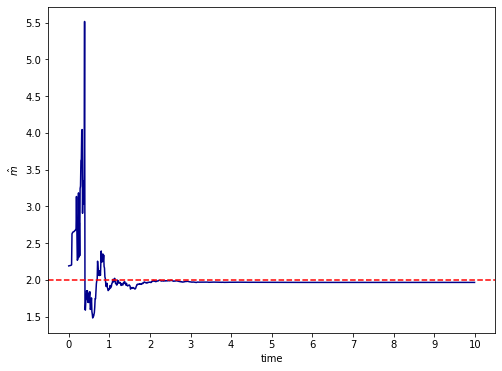
\includegraphics[width=\textwidth]{mOverTime.png}
    \caption{Comparison between $\hat{m}_{Newt}$ and $m$ when $T \rightarrow \infty$}
    \label{fig:f3}
  \end{subfigure}
  \caption{Consistency property for $\sigma$, $\alpha$, and $m$ when $T \rightarrow \infty$}
  \label{fig:consistency}
\end{figure}



{\color{red} The above graphs show the evolution of estimators with a truncated trajectory at time $T$ (Code 1)}

\section{Application to real data}\label{sec-appl}




\subsection{Data description}

We are interested in modeling the biological growth of ......




\subsection{Results}



\section{Conclusions} \label{sec-Conclusions}


\appendix

\section{Proof of consistency and asymptotical normality}



We now study the properties of the estimator $\hat{\alpha}_{ML}$. 
\begin{theorem}\label{Th-consi-norm}
The estimator $\hat{\alpha}_{ML}$ is strongly consistent, i.e.
\begin{equation}\label{consistency}
\lim_{T \rightarrow \infty} \hat{\alpha}_{ML} = \alpha, \qquad \mbox{with probability one}
\end{equation}
and asymtotically normal, i.e.
\begin{equation}\label{normality}
\lim_{T \rightarrow \infty} C_T\Big( \hat{\alpha}_{ML} - \alpha\Big) = \mathcal{N}(0,\sigma^2), \qquad \mbox{in distribution}
\end{equation}
where 
$$
C_T:=\sqrt{Var\left( \int_0^T \big(1-X(t)^m\big)  dB(t)  \right)}
$$
\end{theorem}
\begin{proof}
Observe that using the definition of the SDE \eqref{SGLDE} into \eqref{MLE-alpha} we have
\begin{align}
\hat{\alpha}_{ML} &=\frac{1}{\int_0^T(1-e^{m\sigma Y_t})^2dt}\sigma \int_0^T(1-e^{m\sigma Y_t})\lc\lp \frac{\alpha}{\sigma}\left(1-\exp \lc m\sigma Y(t)\rc \right)-\frac{\sigma}{2}\rp dt+dB(t)\rc\nonumber\\
&\quad+\frac{1}{\int_0^T(1-e^{m\sigma Y_t})^2dt}\frac{\sigma^2}{2}\int_0^T(1-e^{m\sigma Y_t})dt \nonumber\\
&=\frac{\alpha\int_0^T(1-e^{m\sigma Y_t})^2dt}{\int_0^T(1-e^{m\sigma Y_t})^2dt}-\frac{\frac{\sigma^2}{2}\int_0^T(1-e^{m\sigma Y_t})dt}{\int_0^T(1-e^{m\sigma Y_t})^2dt}+\frac{\sigma\int_0^T(1-e^{m\sigma Y_t})dB(t)}{\int_0^T(1-e^{m\sigma Y_t})^2dt}\nonumber\\
&\quad+\frac{\frac{\sigma^2}{2}\int_0^T(1-e^{m\sigma Y_t})dt}{\int_0^T(1-e^{m\sigma Y_t})^2dt}\nonumber\\
&= \alpha+\frac{\sigma\int_0^T(1-e^{m\sigma Y_t})dB(t)}{\int_0^T(1-e^{m\sigma Y_t})^2dt}
%\hat{r}_{ML} &= \frac{1}{\int_0^T  \big( 1-P(t) \big)^2 dt  }  \int_0^T \frac{\big( 1-P(t) \big)}{ P(t)} \Big[ r P(t) [1-P(t) ] dt + \sigma P(t) dB(t)  \Big] \nonumber\\
%&= \frac{r}{\int_0^T  \big( 1-P(t) \big)^2 dt  }  \int_0^T \frac{\big( 1-P(t) \big)}{ P(t)}  P(t) [1-P(t) ] dt  \nonumber\\
%&\qquad +  \frac{1}{\int_0^T  \big( 1-P(t) \big)^2 dt  } \int_0^T \frac{\big( 1-P(t) \big)}{ P(t)}  \sigma P(t) dB(t)   \nonumber\\
%& = \frac{r}{\int_0^T  \big( 1-P(t) \big)^2 dt  }  \int_0^T \big(1-P(t) \big)^2 dt +     \frac{\sigma }{\int_0^T  \big( 1-P(t)\big)^2 dt  } \int_0^T  \big( 1-P(t) \big)  dB(t)   \nonumber\\
%&= r + \frac{\sigma }{\int_0^T  \big( 1-P(t) \big)^2 dt  } \int_0^T  \big( 1-P(t) \big)  dB(t),
\end{align}
then, 
\begin{equation}\label{MLE-r1}
\hat{\alpha}_{ML} - \alpha = \sigma \frac{1 }{\int_0^T(1-e^{m\sigma Y_t})^2dt } \int_0^T(1-e^{m\sigma Y_t})dB(t)
\end{equation}
Then, to prove the result we need to study the right side of \eqref{MLE-r1} without the constant $\sigma$.

Focus on the right term in the equality \eqref{MLE-r1}. We can rewrite it as 
$$
\frac{\int_0^T  \big( 1-e^{m\sigma Y_t} \big)  dB(t) }{Var\left(\int_0^T  \big( 1-e^{m\sigma Y_t} \big) dB(t) \right)  } \times \frac{Var\left(\int_0^T  \big( 1-e^{m\sigma Y_t} \big) dB(t) \right)  } {\int_0^T  \big( 1-e^{m\sigma Y_t} \big)^2  dt }=: \Q_1(T) \times \Q_2(T)
$$

We now study the term $\Q_1(T)$. By taking first and second moment we have that 
\begin{align*}
\E& \int_0^T  \big( 1-e^{m\sigma Y_t} \big)  dB(t) =0\\
Var&\int_0^T  \big( 1-e^{m\sigma Y_t} \big)  dB(t)=\E \left( \int_0^T  \big( 1-e^{m\sigma Y_t} \big)  dB(t) \right)^2 = \E \int_0^T  \big( 1-e^{m\sigma Y_t} \big)^2  dt,
\end{align*}
therefore, $\Q_1(T)$ has zero mean and variance equal to 1 for all $T>0$. From, this we deduce that 
$$
\lim_{T\ \rightarrow \infty} \Q_1(T) = 0, \qquad \mbox {in } L^2,
$$
which implies that 
$$
\lim_{T\ \rightarrow \infty} \Q_1(T) = 0, \quad \mbox {in probability}.
$$
For $\Q_2(T)$. We consider the random variable $1/\Q_2(T)$ and calculate the first moment,
$$
\E\left|\frac{1}{\Q_2(T)} \right| = \frac{\E \int_0^T  \big( 1-e^{m\sigma Y_t} \big)^2  dt }{{Var\left(\int_0^T  \big( 1-e^{m\sigma Y_t} \big) dB(t) \right)  } } = 1 , \quad \mbox {for all } T>0,
$$
From this we have the limit  
$$ 
\lim_{T\ \rightarrow \infty} \frac{1}{\Q_2(T)} = 1,  \qquad \mbox {in } L^1,
$$
and from this expression we deduce that
$$ 
\lim_{T\ \rightarrow \infty} \Q_2(T) = 1,  \qquad \mbox {in } L^1,
$$
which implies that 

$$
\lim_{T\ \rightarrow \infty} \Q_2(T) = 1, \quad \mbox {in probability}.
$$
Finally, by the Slutsky's theorem we conclude that 
$$
\lim_{T\ \rightarrow \infty} \Q_1(T) \Q_2(T) = 0, \quad \mbox {in probability}.
$$
which proves \eqref{consistency}.

To show normality, we note that 

$$
\E\left(\int_0^T  \big( 1-e^{m\sigma Y_t} \big)  dB(t) \right)^2= \E\int_0^T  \big( 1-e^{m\sigma Y_t}   \big)^2 dt 
$$
for all $T>0$, and we deduce from this that
$$
\lim_{T \rightarrow \infty} \frac{1}{\E\int_0^T  \big(1-e^{m\sigma Y_t} \big) ^2dt } \int_0^T  \big( 1-e^{m\sigma Y_t} \big)  dB(t)  = 1, \qquad \mbox {in } L^2 ,
$$
which implies 
$$
\lim_{T\ \rightarrow \infty}  \frac{1 }{ \E\int_0^T  \big( 1-e^{m\sigma Y_t} \big)^2 dt  } \int_0^T  \big( 1-e^{m\sigma Y_t} \big)  dB(t)  = 1, \qquad \mbox {in probability},
$$
Therefore, for the central limit theorem for martingales, we have that 
$$
\lim_{T\ \rightarrow \infty}  \frac{1 }{\sqrt{ \E\int_0^T  \big( 1-e^{m\sigma Y_t}\big)^2 dt }  } \int_0^T  \big( 1-e^{m\sigma Y_t} \big)  dB(t)  = \mathcal{N}(0,1), \qquad \mbox {in distribution},
$$
Moreover, since 
$
\lim_{T\ \rightarrow \infty} \Q_2(T) = 1, \quad \mbox {in probability}.
$
and by the Slutsky's theorem we conclude that 
$$
\lim_{T\ \rightarrow \infty} \big( \hat{\alpha}_{ML} - \alpha \big ) = \mathcal{N}(0,\sigma^2), \qquad \mbox {in distribution}.
$$
which proves \eqref{normality}.
\end{proof}

\begin{thebibliography}{999}

\bibitem{be-sm-00} J.M. Bernardo, A.F.M Smith. Bayesian Theory.  John Wiley and Sons, Ltd. (2006). 

\bibitem{bl-so-14} M. Bladt and M. S\o rensen. Simple simulation of diffusion bridges with application to likelihood inference for diffusions, Bernoulli 20 645–675 (2014).
\bibitem{br-go} Braun, M.,  Golubitsky, M.  Differential equations and their applications (Vol. 1). New York: Springer-Verlag. (1983).


\bibitem{bu-fa} R.L. Burden, D.J. Faires: Numerical Analysis (7th ed.). Brooks/Cole. (2000).

\bibitem{co-pa} S. Corlay, G. Pag s: {\it Functional quantization based stratified sampling methods}. Monte Carlo Methods and Applications, Volume 21, Issue 1, Pages 1–32, ISSN (Online) 1569-3961, ISSN (Print) 0929-9629. (2015).

%\bibitem{co-na-19} J.-C. Cort\'es, A. Navarro-Quiles, J.-V. Romero, M.-D. Rosell\'o: {\it  Analysis of random non-autonomous logistic-type differential equations via the Karhunen-Lo\'eve expansion and the Random Variable Transformation technique}.
%Communications in Nonlinear Science and Numerical Simulation. Volume 72, Pages 121-138, (2019).

\bibitem{ge-ca-13} A. Gelman, J. B. Carlin, H. S. Stern, D. B. Dunson, A. Vehtari, D.B Rubin: Bayesian Data Analysis. Chapman and Hall/CRC Texts in Statistical Science (2013).

\bibitem{gh-sp}  R.G. Ghanem, P.D. Spanos: Stochastic Finite Elements: A Spectral Approach. Springer, New York, (1991).


\bibitem{gh-de-06} J. K. Ghosh, M. Delampady, T. Samanta: An Introduction to Bayesian Analysis Theory and Methods. Springer Texts in Statistics. (2006). 

\bibitem{iacus} Iacus, S. M. Simulation and inference for stochastic differential equations: with R examples. Springer Science \& Business Media. (2009).

\bibitem{ji-shi} Jiang, D., Shi, N. A note on nonautonomous logistic equation with random perturbation. Journal of Mathematical Analysis and Applications, 303(1), 164-172. (2005). 

\bibitem{kl-pl} Kloeden, P. E.,  Platen, E.  Numerical solution of stochastic differential equations (Vol. 23). Springer Science \& Business Media. (2013).


\bibitem{li-sh} Liptser, R. S., Shiryaev, A. N.  Statistics of random processes: I. General theory (Vol. 1). Springer Science \& Business Media. (2001).

\bibitem{lo-po} G. J. Lord, C.E. Powell, T. Shardlow:  An Introduction to Computational Stochastic PDEs
Cambridge Texts in Applied Mathematics. (2014)
\bibitem{mc-kr-97} McLachlan,G.J.,Krishnan,T.The EM Algorithm and Extensions. Wiley, NewYork(1997).

\bibitem{panik} Panik, M. J.  Stochastic Differential Equations: An Introduction with Applications in Population Dynamics Modeling. John Wiley \& Sons. (2017).


\bibitem{pr} P. Protter: Stochastic integration and differential equations, Springer-Verlag, Berlin, (2004).

\bibitem{su} Suryawan, H. P. (2018). {\it Analytic solution of a stochastic richards equation driven by Brownian motion}. In Journal of Physics: Conference Series (Vol. 1097, No. 1, p. 012086). IOP Publishing.

\bibitem{wei} Wei-Cheng, M. {\it Estimation of diffusion parameters in diffusion processes and their asymptotic
normality}, Int. J. Contemp. Math. Sci. 1, 763–776 (2006).
\bibitem{Bevia2023}
V.~Bevia, J.~Calatayud, J.-C. Cortés, and M.~Jornet.
\newblock {On the generalized logistic random differential equation:
  Theoretical analysis and numerical simulations with real-world data}.
\newblock {\em Communications in Nonlinear Science and Numerical Simulation},
  116:106832, 2023.

\bibitem{Braumann2008}
Carlos~A. Braumann.
\newblock {Growth and extinction of populations in randomly varying
  environments}.
\newblock {\em Computers \& Mathematics with Applications}, 56(3):631--644,
  2008.

\bibitem{Cortes2019}
J.-C. Cortés, A.~Navarro-Quiles, J.-V. Romero, and M.-D. Roselló.
\newblock {Analysis of random non-autonomous logistic-type differential
  equations via the Karhunen–Loève expansion and the Random Variable
  Transformation technique}.
\newblock {\em Communications in Nonlinear Science and Numerical Simulation},
  72:121--138, 2019.

\bibitem{Liu2013}
Meng Liu and Ke~Wang.
\newblock {A note on stability of stochastic logistic equation}.
\newblock {\em Applied Mathematics Letters}, 26(6):601--606, 2013.

\bibitem{Schurz2007}
Henri Schurz.
\newblock Modeling, analysis and discretization of stochastic logistic
  equations.
\newblock {\em Int. J. Numer. Anal. Model.}, 4(2):178--197, 2007.



%\bibitem{zh-ka}  Z. Zhang, G. Karniadakis: Numerical Methods for Stochastic Partial Differential Equations with White Noise. Springer, Berlin (2017)
\end{thebibliography}
\end{document}

 